\documentclass{article}

\usepackage{lipsum}
\usepackage[margin=1in,includefoot]{geometry}
\usepackage{graphicx}
\usepackage{float}
\usepackage[hidelinks]{hyperref}
\usepackage{amsmath}
\usepackage{amssymb}

% Header and Footer Stuff
\usepackage{fancyhdr}
\pagestyle{fancy}
\fancyhead{}
\fancyfoot{}
\fancyfoot[R]{\thepage}
\renewcommand{\headrulewidth}{0pt}
\renewcommand{\footrulewidth}{0pt}

\begin{document}

\begin{titlepage}
	\begin{center}
	\begin{align*}
	
\includegraphics[height=1.75in]{logo.png}
	\end{align*}


	
	\line(1,0){300}\\
	[0.25in]
	\huge{\bfseries The Fourier Analysis}\\
	[2mm]
	\line(1,0){200}\\
	[1.5cm]
	\textsc{\LARGE Laboratory D2}\\
	[0.75cm]
	\textsc{\Large 3C2 Digital Circuits}\\
	[7cm]	
	\end{center}
	
	
	
	\begin{flushright}
	\textsc{\large Alexandru Sulea\\
	D Stream\\
	\#12315152\\
	16 December 2015\\}
	\end{flushright}

\end{titlepage}
%Table of Contents Stuff%
\tableofcontents
%\listoffigures
%\addcontentsline{toc}{section}{List of Figures}
\listoftables
\addcontentsline{toc}{section}{List of Tables}


\thispagestyle{empty}
\cleardoublepage
\pagenumbering{arabic}
\setcounter{page}{1}


\section{Introduction}\label{sec:intro}
The following lab is designed to further improve our knowledge of 
semi-conductors and MOS transistors. The lab encompasses the wave synthesis of circuit signals comprised of MOS components.  The D2 lab also composes the second part of the Multisim introduction tutorial. Following on the previous established standards of lab D1, this lab encompasses more of the MultiSim simulation and analytic power.\\
In this lab the static and dynamic characteristics which affect the performance of CMOS electronics will be explored and documented in depth.(ref 3.)\\

\section{Theory}\label{sec:theory}
\subsection{A. MOS Transistor Characteristics}
One of the most widely used electronic components in digital integrated circuits is the metal-insulated-transistor or more commonly referred to as MIS. A determining factor of this component is that the channel current is controlled by a voltage applied at the gate electrode that is isolated from the channel by an insulator.(Ref 4.)\\

Although MIS is the most accurate description, since most devices use silicon in their composition the term  MOSFET or metal–oxide–semiconductor field-effect transistor is more commonly used.\\

Silicon is more commonly used than other better rare metal alternatives due to the wide availability of silicon on Earth and the relatively cheap and simple process of producing silicon wafers.\\
 

The MOS transistor is a semiconductor made in two variations , either n-p-n or p-n-p, The semiconductor material being layered like a sandwich to achieve the desired semiconducting attribute.\\


The N-channel MOS transistor is comprised  of two outer layers of n-type silicon. One side is the Source while the other acts as the drain. Sandwiched in between the two n-type layers there is a thin slice of p-type silicon substrate which acts as the Gate. The Source and Drain are not physically connected between themselves, thus no current flow passes from one to the other without first passing through the p-type silicon gate.  Hence the name n-p-n.\\

The P-channel MOS transistor is comprised in turn of two outer layers of p-type silicon. One of the p-type sides acting as the Source while the other acts as the drain. Sandwiched in between the two p-type layers there is a thin slice of n-type silicon substrate which acts as the Gate. The Source and Drain are again not physically connected between themselves and as in the previous paragraph there is no current flow between Source and Drain without first passing through the gate.  Hence the name p-n-p.\\

The MOS transistor is evaluated with theoretical formulas but the conductivity of the material is based in real life factors such as the purity of the material and the dimensions of the transistor.\\
The level of purity in the material will indicate the efficiency and operational lifetime of a transistor. The higher the purity the better the transmission of current and the longer the transistor will last. \\
The dimensions also play a key role as if the gate is too narrow the current may jump from source to drain creating a short in the circuit. Then again if the dimension is too large it may be very difficult to transfer current across from source to drain.\\ 



One view of MOSFET is that it is a gate-controlled potential barrier or resistor.(Ref 2. )

\subsection{B. Restively Loaded MOS Transistor Inverter}
As the title implies, this version of the MOS transistor is resistevely loaded to give it an inverting capability. The circuit is not comprised of one individual component , but multiple electronic components working in tandem. \\
The circuit includes a resistor to absorb some of the current being sent into the p-type transistor. The final part is that the output feeds back into itself thus inverting whatever was sent before. Hence the name resistevely loaded inverter.

\subsection{C. The CMOS Inverter}
CMOS or complementary metal–oxide–semiconductor is a subset of the MOSFET digital electronic component family. CMOS only MOS is not a different component in itself, but refers to the use of n-type and p-type transistors to make a NOT gate.\\
As the name implies it uses complimentary pairs of transistors. A CMOS gate is essentially a p-type and n-type transistors linked together to form a NOT gate, thus inverting any signal received from a 0 to a 1.\\
\begin{align*}
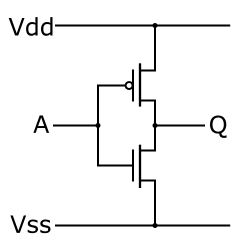
\includegraphics[height=1.75in]{D2S0.png}
\end{align*}\\
(Ref 5.)


\pagebreak
\section{Results}\label{sec:result}
\subsection{A. MOS Transistor Characteristics}




\begin{table}[H]
\centering
\caption{Model Table}
\label{my-label}
\begin{tabular}{|l|l|l|}
\hline
 & n-channel & p-channel \\ \hline
length & 1um & 1um  \\ \hline
width & 2um & 4um \\ \hline
vto & 1V & -1V \\ \hline
kp & $2e^{-005}A/V^{2}$ & $1^e{-005}A/V^{2}$  \\ \hline
\end{tabular}
\end{table}


\begin{align*}
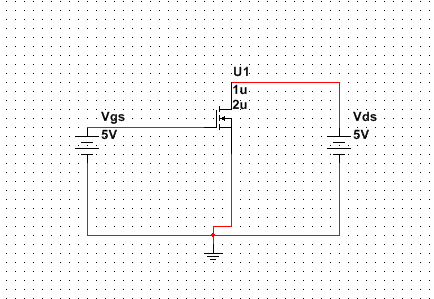
\includegraphics[height=1.75in]{D2P1.PNG}
\end{align*}\\

Q.10
\begin{align*}
\centering
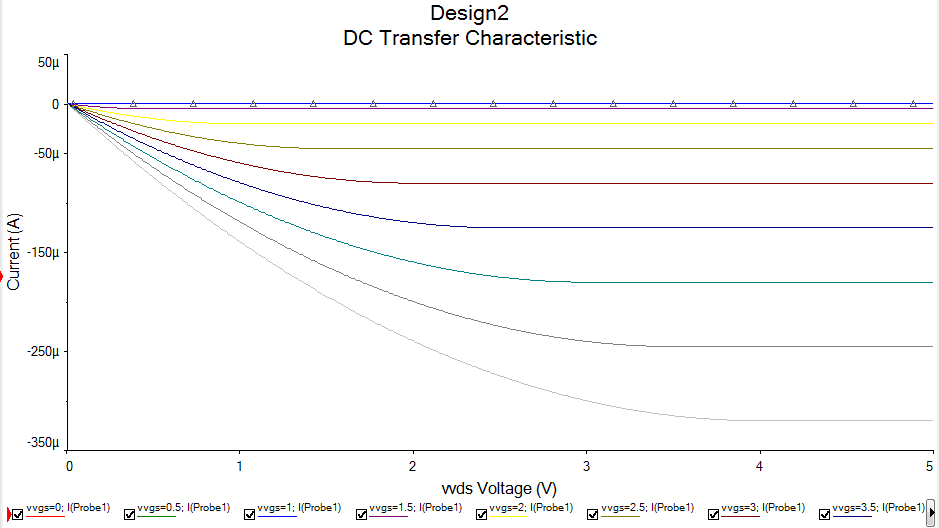
\includegraphics[height=1.75in]{D2P2.PNG}
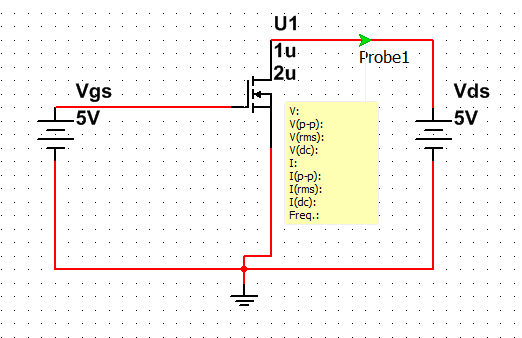
\includegraphics[height=1.75in]{D2P3.PNG}
\end{align*}\\
Q13.
\begin{align*}
\centering
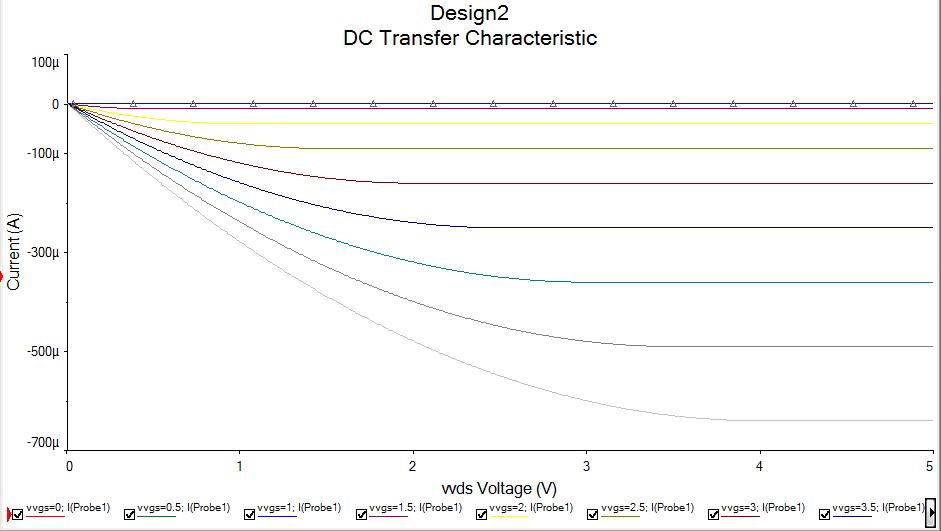
\includegraphics[height=1.75in]{D2P4.PNG}
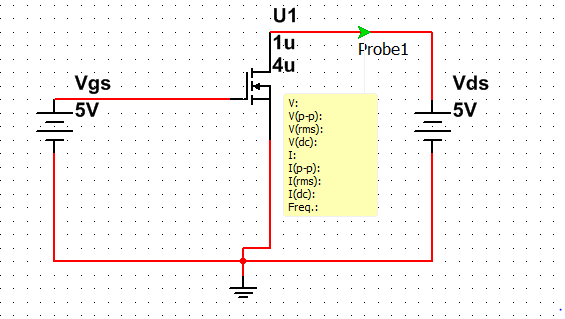
\includegraphics[height=1.75in]{D2P5.PNG}
\end{align*}\\
\subsection{B. Resistevely Loaded MOS Transistor Inverter}

$$ V_{O}=V_{L}=\left( V_{DD}-V_{T}+\frac{1}{(K_{n})(R_{L})}\right)\pm \sqrt{\left( V_{DD}-V_{T}+\frac{1}{(K_{n})(R_{L})}\right)^{2}-\frac{V_{DD}}{(K_{n})(R_{L})}} $$

Using the above formula the value for $V_{O}=7.5V$ or $0.3V$ if the fixed resistor has a value of $100K\Omega$ 



Q6.
\begin{align*}
\centering
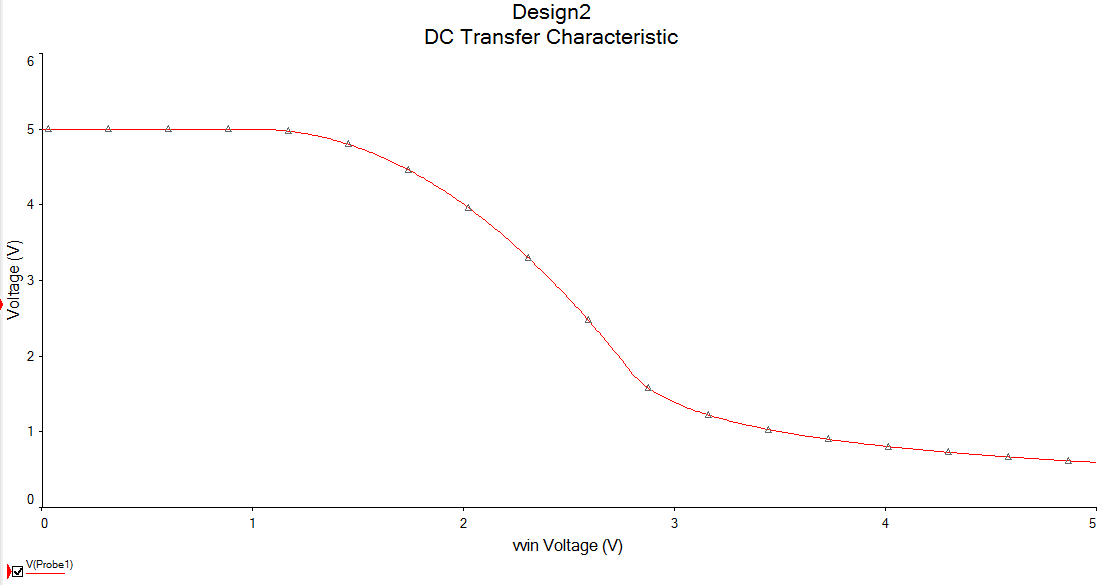
\includegraphics[height=1.75in]{D2P6.PNG}
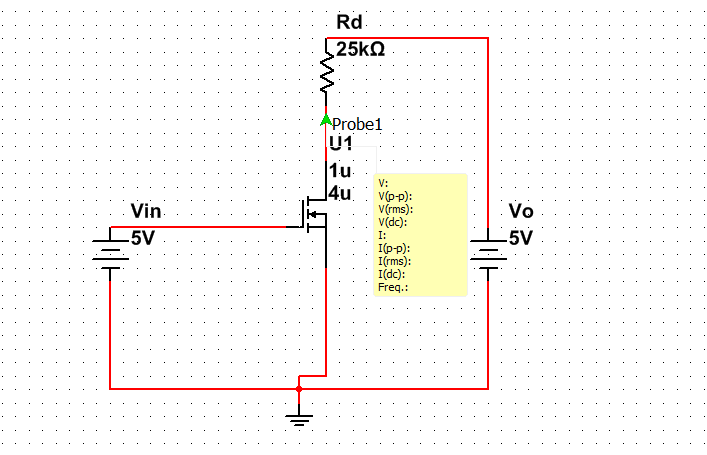
\includegraphics[height=1.75in]{D2P7.PNG}
\end{align*}\\
The values in the simulation are somewhat less than the values obtained in the lectures. This is due to the fact that the simulation gives an approximation of the real life values and the lecture provides the ideal values.\\



Q7. and Q8.
\begin{align*}
\centering
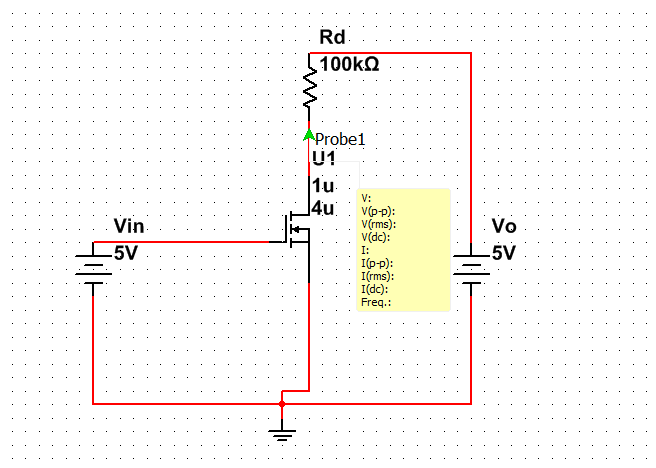
\includegraphics[height=1.75in]{D2P8.PNG}
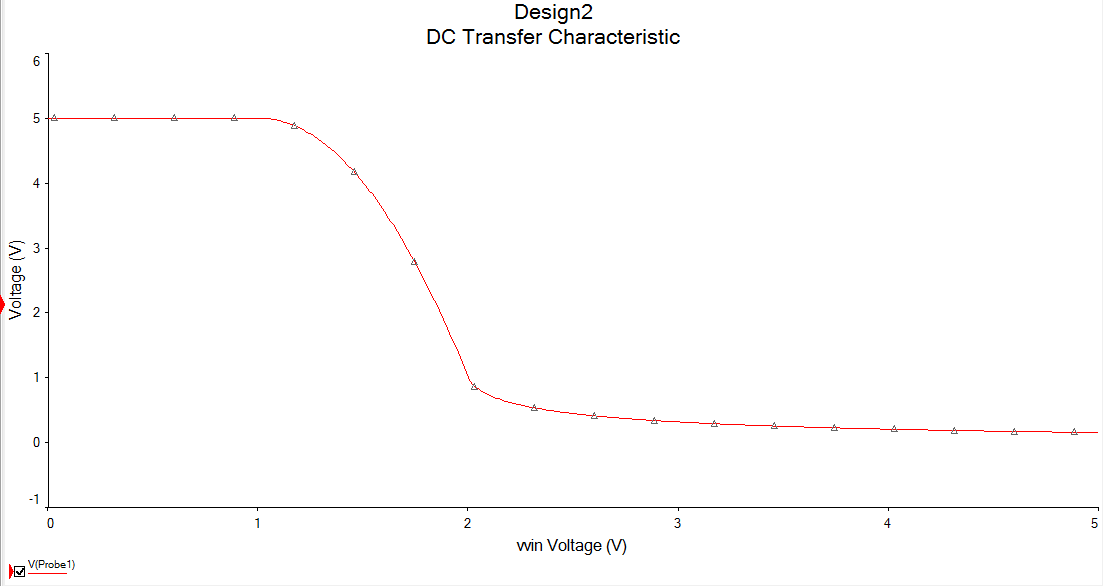
\includegraphics[height=1.75in]{D2P9.PNG}
\end{align*}\\

Q9.
\begin{table}[H]
\centering
\caption{My caption}
\label{my-label}
\begin{tabular}{|l|l|}  \hline
$V_{ILmax}$ & 1V \\ \hline
$V_{IHmin}$ & 2V \\ \hline
$V_{OL}$     & 1V  \\ \hline
$V_{OH}$     & 5V \\ \hline
\end{tabular}
\end{table}

Q10.
\begin{align*}
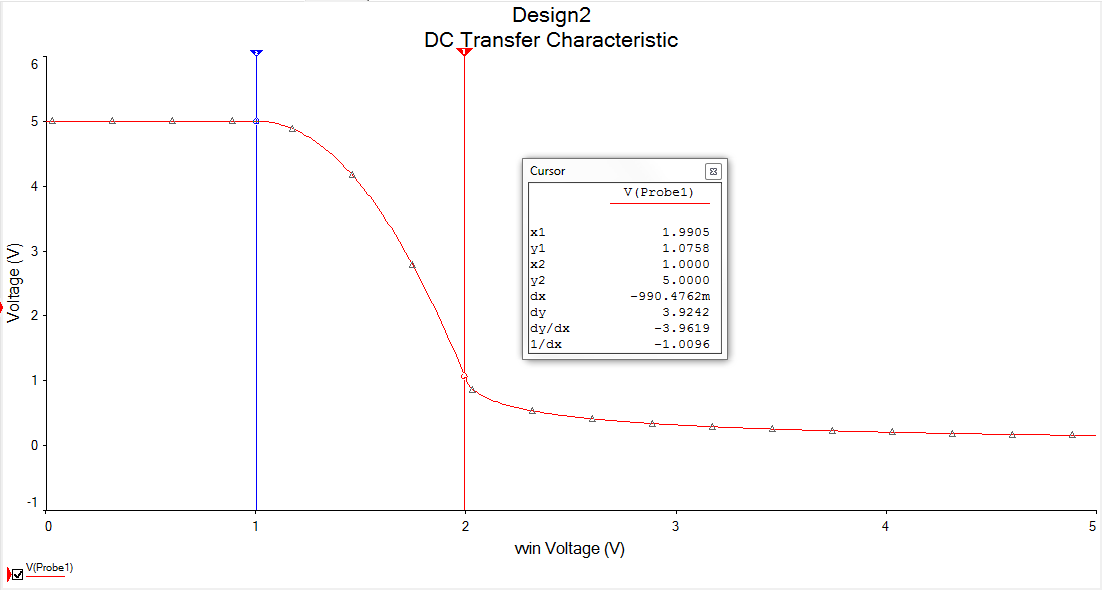
\includegraphics[height=1.75in]{D2P10.PNG}
\end{align*}\\

\subsection{C. The MOS Inverter}
\subsubsection{C.1 Static Characteristics}
Q3.
\begin{align*}
\centering
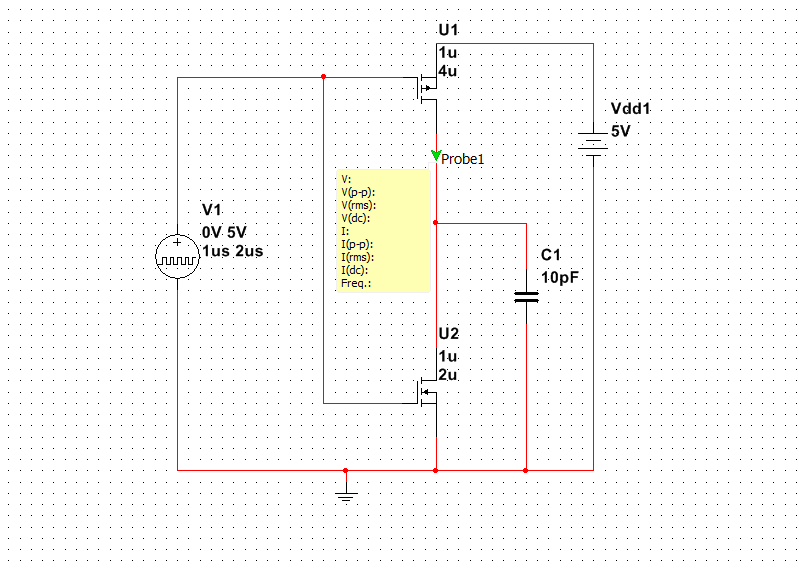
\includegraphics[height=1.75in]{D2P12.PNG}
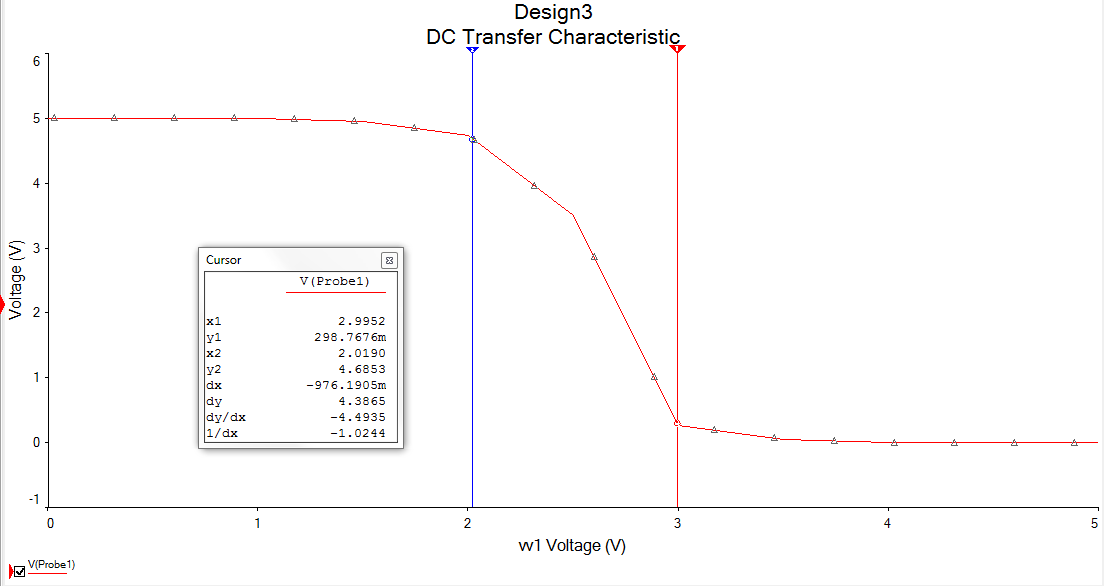
\includegraphics[height=1.75in]{D2P13.PNG}
\end{align*}\\

Q4.
\begin{table}[H]
\centering
\caption{My caption}
\label{my-label}
\begin{tabular}{|l|l|}  \hline
$V_{ILmax}$ & 2V \\ \hline
$V_{IHmin}$ & 3V \\ \hline
$V_{OLmax}$ & 0.3V \\ \hline
$V_{OHmin}$ & 4.6v \\ \hline
\end{tabular}
\end{table}


\subsubsection{C.2 Dynamic Performance}

Q6.
\begin{table}[H]
\centering
\caption{My caption}
\label{my-label}
\begin{tabular}{|l|l|}  \hline
$t_{PHL}$ & 0.0874us \\ \hline
$t_{PLH}$ & 0.0715us \\ \hline
$t_{f}$ & 0.1906us \\ \hline
$t_{r}$ & 0.2065us \\ \hline
\end{tabular}
\end{table}
Q7.
\begin{align*}
\centering
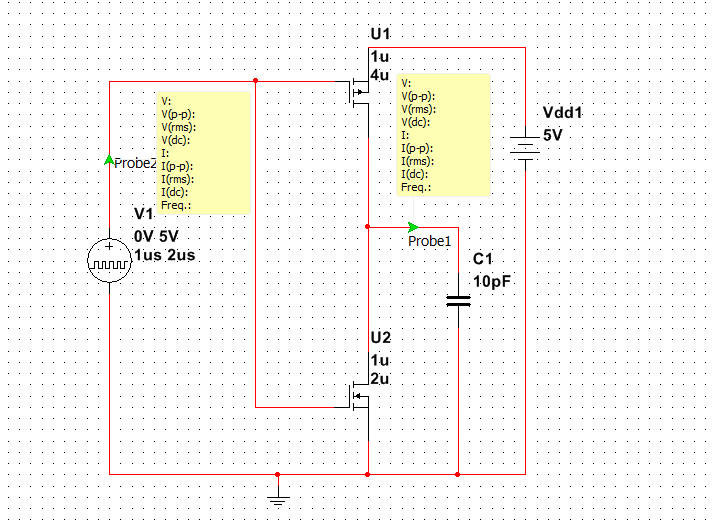
\includegraphics[height=1.75in]{D2P14.PNG}
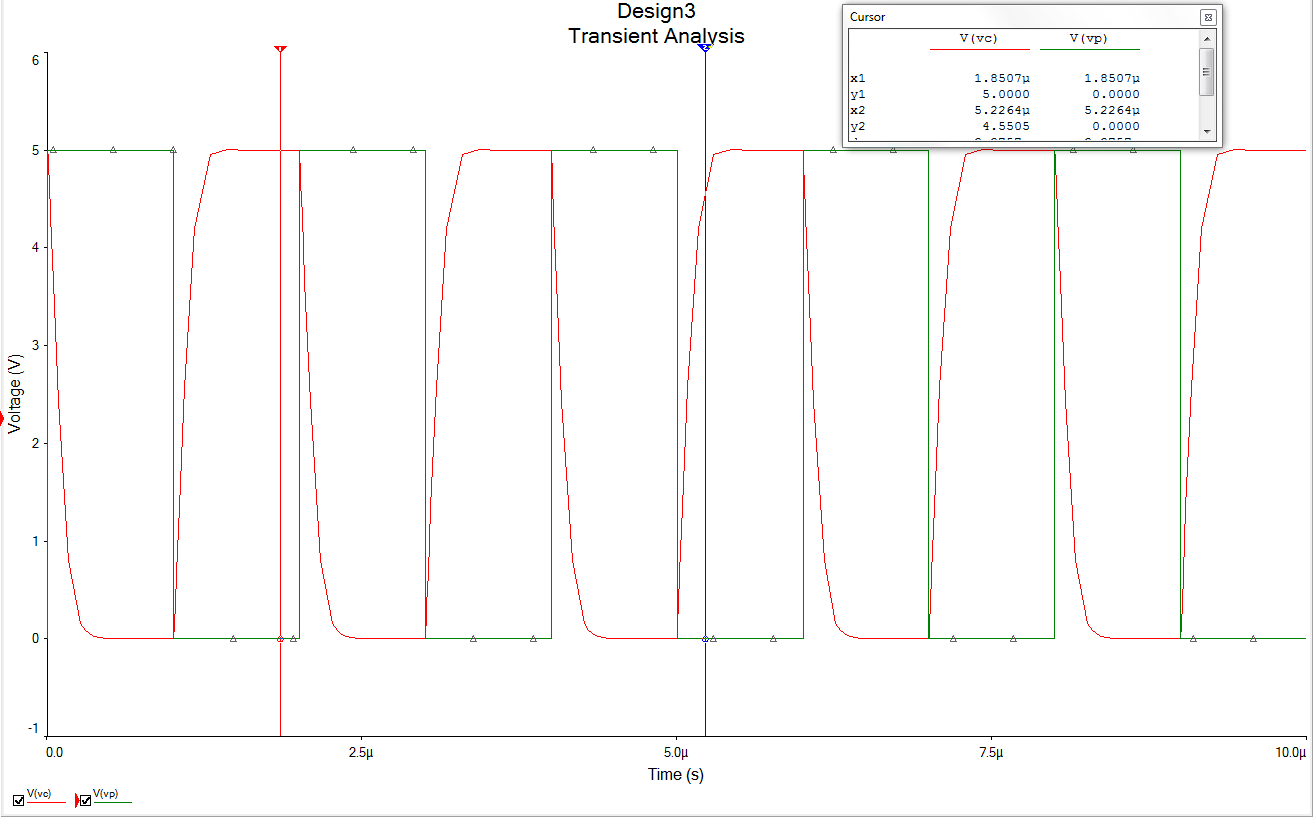
\includegraphics[height=1.75in]{D2P15.PNG}
\end{align*}\\




\pagebreak

\begin{flushleft}
\section{Discussion}\label{sec:discuss}\underline{}


Q1. What are the limitations on the accuracy of your results?\\
A1. The Multisim graph is only accurate within 0.5s of the actual value. As seen in the pictures shown, we were never able to receive a conclusive absolute 90percent value, but we were able to get within a significant enough approximation of that value.\\
The second limitation, and it is a limitation shared by all simulation software is that there can never be enough variables tested in the simulation to give a real world scenario data. \\
The data and graphs observed in the Multisim simulation are simply an approximation and a midway point between the ideal values and the real world values. \\
Q2. How do the values of parameters compare with those obtained in lectures?\\
A2. The values of the parameters were not similar to those obtained in the lectures, as can be seen from the graphs also , they have a less than ideal curve to them. The values obtained in the simulation are also not the values one would observe in a real life situation. Thus the values obtained in this lab are somewhere in between real-life values and the ideal ones.\\
Q3. What are the advantages or disadvantages of circuit simulation such as those carries out in the experiments?\\
A3. The benefits of the Multisim simulation is that it allows for a broad range of component libraries to be searched and a circuit to be assembled in a very short amount of time.
Being a Simulator, it also allows for a quick and accurate simulation of the selected circuit with a broad range of analytic tools to be applied to the circuit for observation.\\
If a mistake is made during the simulation or if a component needs to be altered , the entire circuit can be edited and reapplied in a very short amount of time with no extra cost what so ever. \\
The Disadvantages of the Multisim simulation is that while it offers a broad range of libraries , it also confines the user within those libraries. It thus however cannot simulate anything new or experimental that hasn't been added to the library. The scale of the simulation is also limited to a small number of circuits, The multisim simulation cannot simulated the entire circuitry involved in a complicated machine all at once. Thus a large circuit has to be broken down into smaller pieces, all simulated in a row.
Q4. What are the benefits or drawbacks of circuit simulation and of Multisim in general as applied to the design of electronic circuits?\\
A4. the benefits of circuit simulation are of course that it is quick and cheap, with absolutely no drawbacks in experimenting with a new wireing system for an electronic concept.\\
The drawbacks are that unlike real life the system cannot simulate the environmental factors which may or may not be an issue for the circuit design. Environmental factors such as vibration temperature and humidity play a big role in almost every big industry , from mining companies to aerospace firms.\\
Q5. What are the essential elements of good circuit simulation and simulators?\\
A5. The essentials of a good simulation would be good planning and design, the requirements of the circuit should be well understood before the circuit is simulated. By knowing this we ensure that there are as few mistakes made an as few versions of the circuit that will have to be reiterated. In some cases, good planning saves a lot of time and effort. \\
Q6. What is the role of the Electronic  Engineer in this regard?\\
A6. The role of an electronic engineer is to be well versed in the standards and practices of electronic component design. To understand the project in depth and also the problem the electronic circuit is to solve.
furthermore the job of an electronic engineer is to understand that the simulation software will only take one so far and that using their knowledge electrical engineering will take the issues into account which the simulator cannot such as environmental factors, cost and lifetime of the circuit. \\
\end{flushleft}


\pagebreak

\section{Conclusion}
Upon completing the laboratory a few decisive conclusions were reached. Multisim is a very handy and thorough simulation, but due to its simplicity it lacks some real world factors which would make a difference in the real world. Thus the results obtained in this lab were merely a rough approximation of the results observer in real life. Thus the Multisim values will always lie somewhere in between the ideal and real world values.
The second conclusion is that by manipulating a small part of a circuit, or electrical components attributes , great differences can be observed. This suits particularly well because it means that the components are not only simple to manufacture and cheap to produce but also flexible in their attributes and applications.
The third and final observation was that CMOS has a large noise margin which can be observed in the experiment by the transition from LO to HI. This is in part a bi-product of MOS characteristics due to a asimetrically  rapid charge build up but a slow charge depletion.


\appendix


	
	\begin{thebibliography}{3}
  %league
  \bibitem{one}
  \emph{3C2 Signals and Systems Notes},
  
  \bibitem{two}
  Chih-Tang Sa,
  \emph{Fundamentals of Solid State Electronics},

  
  \bibitem{three}
  \emph{Lab Description},
  
  
  
  \bibitem{four}
  Ben g. Streetman,  Sanjay Kumar, Banerjee
  \emph{Solid State Electronic Devices},
  Sixth Edition.
  
  %kelly betting
  \bibitem{five}

  \emph{Wikipedia (CMOS picture)},

  
\end{thebibliography}
	
\end{document}